This section describes algorithms and techniques commonly employed in supervised machine learning, specifically in classification problems.
We also discuss the \textit{class imbalance problem}, mentioning and comparing mitigation techniques and elaborating on methods to evaluate results under class imbalance.


\section{Classification Algorithms} \label{sec:classification_algorithms}

Supervised learning consists of extracting knowledge by obtaining patterns from curated domain data.
More specifically, through a process called "training" or "induction" of models, a function that relates independent input variables to a dependant output is approximated.
This is made possible by the fact that in supervised learning the data points are examples of the true mapping from input to output variables.
When the output of the models is categorical (that is, its values are always of a finite set of \textit{classes}) this task is then named supervised learning classification, as opposed to the alternative of continuous values that is named regression.
Thus, these models are useful for their ability to classify or predict new occurrences of a phenomenon, based on the values of the independent variables.
Several algorithms are available for the creation of classification models, each with interesting and important peculiarities.
In this section, we review the ones employed in the methodology of our study.

\subsection{Decision Trees} \label{subsec:decision_trees}

Decision trees (DTs) are widely used in machine learning applications in general~\cite{Kotsiantis2013}, and in the medical domain~\cite{Burke2019}, for their potential for human understanding and classification effectiveness~\cite{Podgorelec2002}.
Instances are classified in decision trees by following a path from the trees' root down to one of its leaves.
At each node, as depicted in Figure~\ref{fig:decision-tree}, the instance has its value for some feature compared to some inducted rule of classification to define the decision path~\cite{Kubat2017}.

The problem of finding the shortest trees with the best rules and tests of variables is approached (though not optimally solved) with different \textit{heuristics}, mainly distinguished by their \textit{node-splitting} criteria (e.g. \textit{information gain}, \textit{gain ratio}, and \textit{Gini value})~\cite{Kotsiantis2013}.
Growth in size and complexity in decision trees tends to lead to losses in interpretability generality, tending to overfit training data, which is the reason why techniques like \textit{pruning} and \textit{feature selection} are applied~\cite{Kotsiantis2013}.

\begin{figure}[H]
    \caption{A depiction of a decision tree}
    \centerline{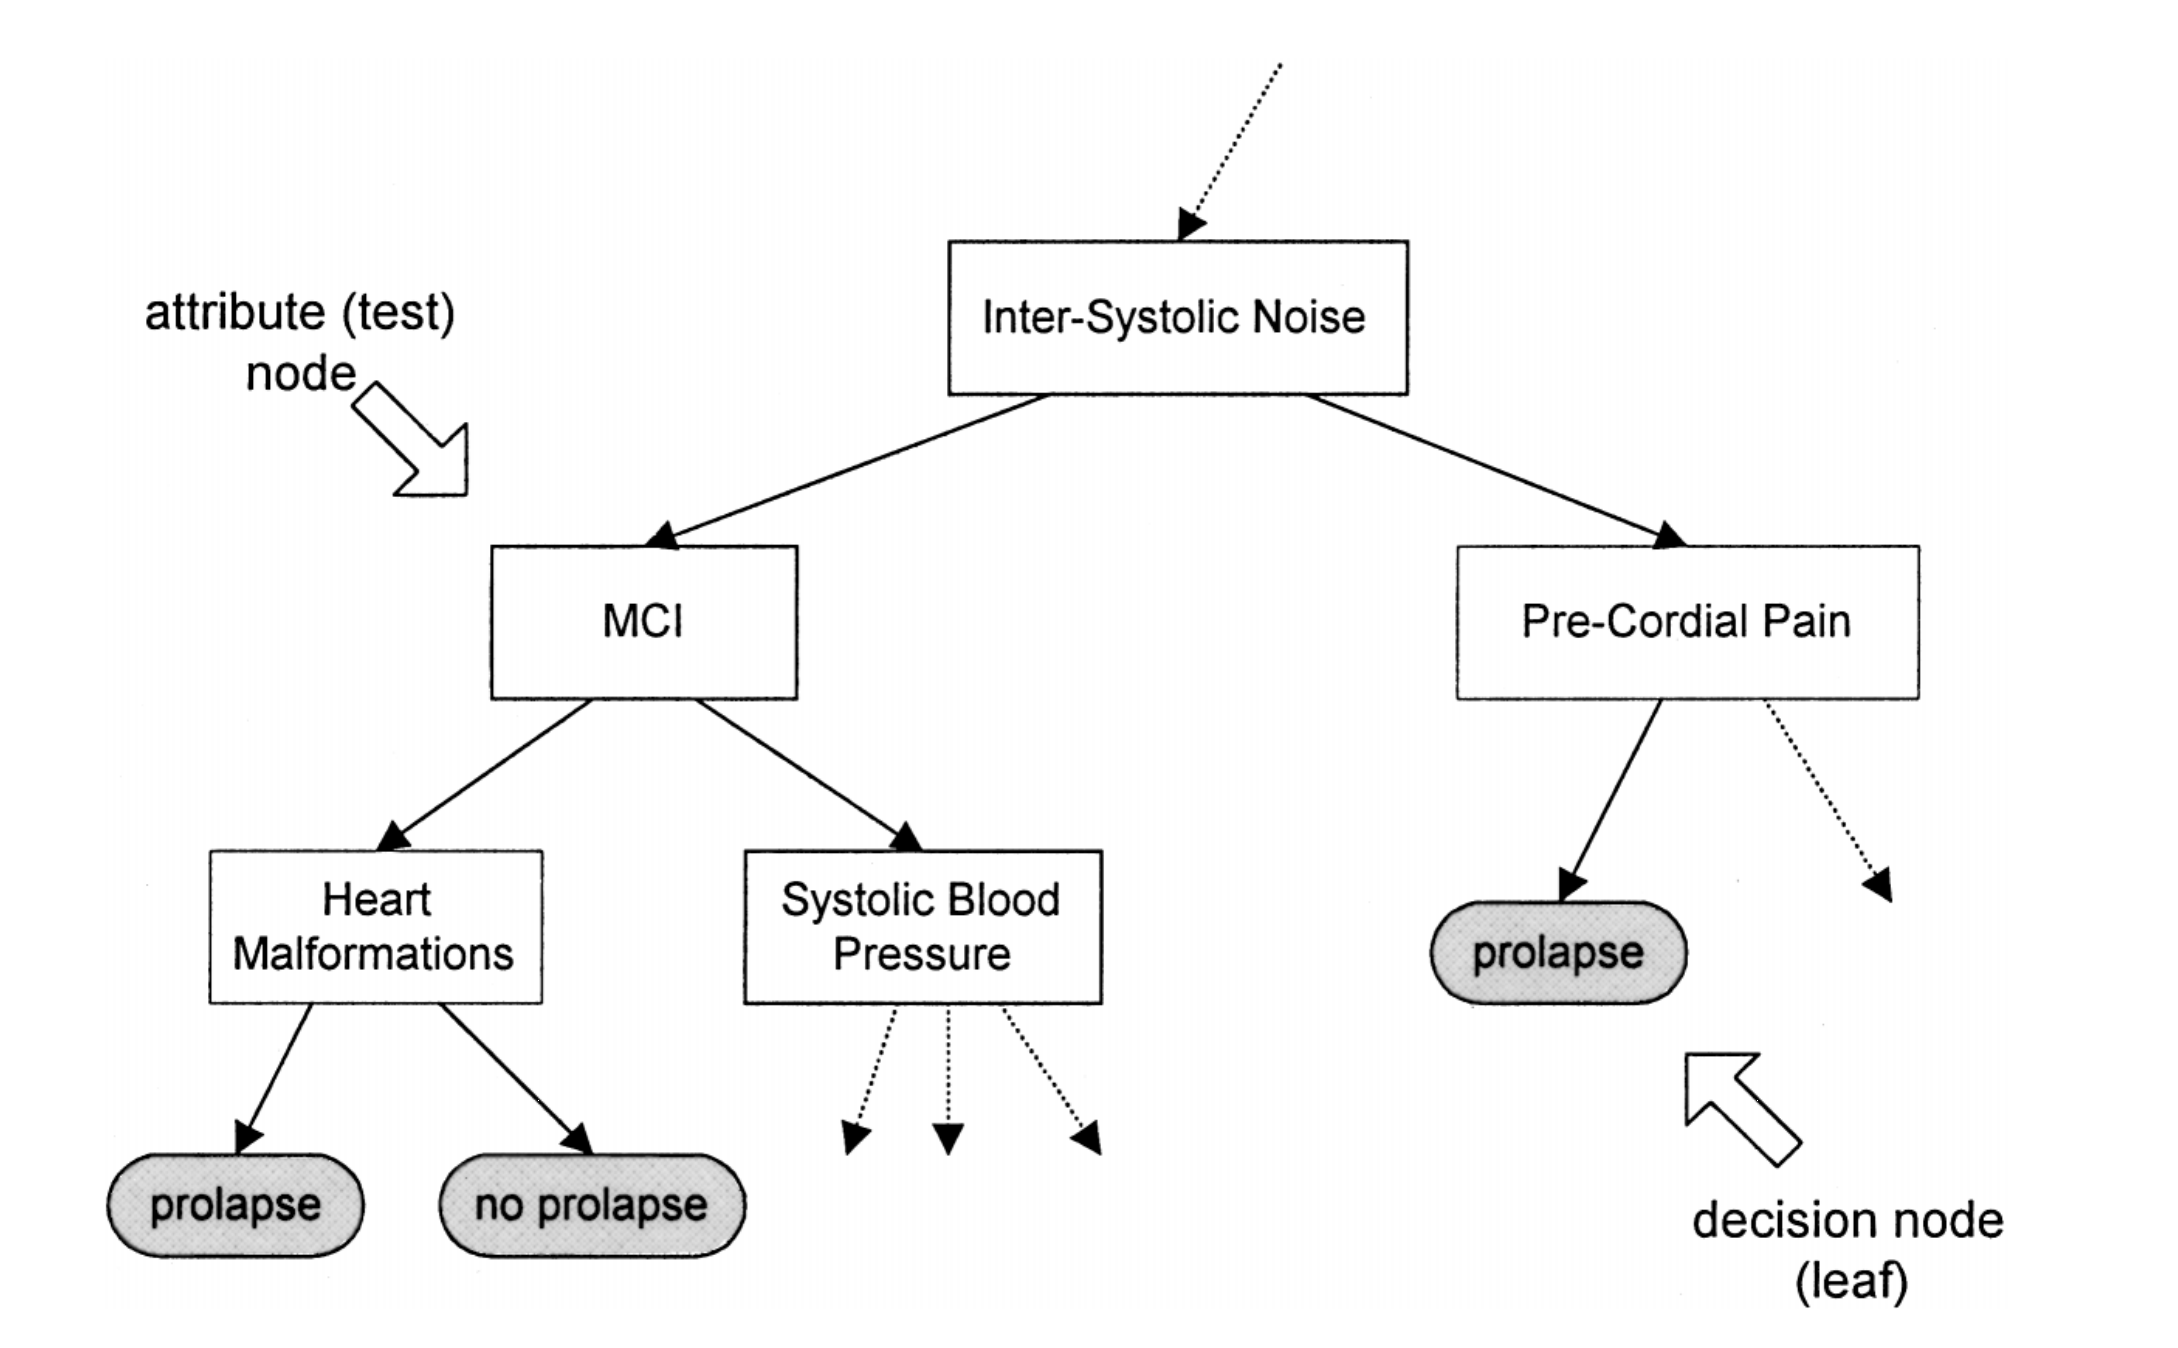
\includegraphics[scale=.4]{fig_decision_tree.png}}
    \label{fig:decision-tree}
    \legend{Source: ~\citet{Podgorelec2002}}
\end{figure}

%\subsection{Adaboost}\label{subsec:adaboost}
%
%\textit{Boosting} is an ensemble induction approach that achieves a similar effect to bagging, but without relying on randomness and the performance of each independently-induced classifier.
%Instead, boosting trains each new predictor based on the shortcomings of its predecessors, so they are correlated by an iterative improvement~\cite{Kubat2017}.
%Originally designed as the aggregate of three classifiers, boosting is adapted by the \textit{Adaboost} algorithm to have many more learners.
%The induction is done by the probabilistic selection of training examples in a way that reinforces ones with more misclassifications each time.
%Moreover, Adaboost uses \textit{weighted majority voting} with decision power (weights) concentrated according to performance~\cite{Kubat2017}.

%\textcolor{red}{\textbf{mention afterwards why not used}}

%\subsection{Support Vector Machines}\label{subsec:svms}
%
%Support Vector Machines (SVMs) are classifiers that find class separation boundaries for problems where there is "class overlap" in feature space (from which simple a linear boundary wouldn't make an accurate separation)~\cite{Hastie2009}.
%SVMs achieve this by transforming (enlarging) the feature space with non-linear \textit{kernel} function to enable higher-dimension hyperplane boundaries to separate the data.
%
%\textcolor{red}{\textbf{mention afterwards why not used}}

\subsection{Elastic Nets}\label{subsec:elastic_nets}

The Elastic Net (EN) is a regularization and feature selection method for linear or logistic regression that essentially combines two other regression methods called ridge and lasso.
It improves on lasso by generalizing it~\cite{Zou2005}.
The technique introduces a \textit{grouping effect} with which correlated variables stick together in regards to their relative contribution to the prediction, which can be estimated for the same usefulness as \textit{p}-values for assessing their importance~\cite{Burke2018}.
The nature of the algorithm begs the definition or selection of two hyperparameters: lambda (the regularization parameter) and alpha (the ridge-lasso-mixing parameter).

\subsection{Artificial Neural Networks}\label{subsec:anns}

Artificial Neural Networks (ANNs) are machine learning algorithms based on a graph structure of nodes (called \textit{neurons}) interconnected by weighted links.
Each neuron calculates an output that is a combination of its inputs (the network actual inputs or the outputs of other neurons) based on linear or non-linear functions.
Arranged in layers, these structures are also called \textit{multilayer perceptrons}, using \textit{forward propagation} to classify instances.
This process in the chain calculation of the neurons' activations up to the \textit{output layer}, where the prediction is decided to be class represented by the neuron with the highest value.
Based on a calculated error, the network updates its weights by the process called \textit{backpropagation}, implementing error minimization by \textit{gradient descent}~\cite{Kubat2017}.
Since ANNs are a large family of algorithms, many hyperparameters can be explored depending on the exact variation employed, but arguably the most basic ones are the number of hidden layers and neurons per in each hidden layer of the network.


\section{Ensemble Learning}\label{sec:ensemble-learning}

Supervised learning algorithms can be grouped to improve prediction performance and robustness, constituting an \textit{ensemble}.
This can be achieved by several different approaches, each with varying degrees of complexity.
The emerging trade-off between lesser interpretability by increased complexity and predictive power should always be considered, as its asymmetry is dependent on the domain, the dataset, and the underlying algorithms involved.
That said, it has been shown that, in general, good results can be achieved with relatively simple combinations of predictors~\cite{Clemen1989}.
Commonly employed techniques of lower complexity include:
\begin{itemize}
    \item majority voting: when the classification outcome is defined by the most predicted class among the ensemble's constituents;
    \item weighted averaging: when the class with the highest linearly-combined probability between constituents is chosen.
\end{itemize}

\subsection{Random Forests}\label{subsec:random_forests}

Random Forests are defined as ensembles of decision trees (grown considering random vectors) that classify instances by majority voting\cite{Breiman2001}.
Random forests are also useful for generating ranks of features importance by assessing the automatically computed variable importance measures (VIMs) of the forest~\cite{Boulesteix2012}.

This ensemble is trained using \textit{bagging}, an acronym for \textit{bootstrapping} and \textit{aggregation} (majority voting).
Bootstrapping works by composing a number of training subsets by sampling from the original training data with replacement, then inducing a tree classifier from each~\cite{Kubat2017}.
This process is illustrated in the left half of Figure~\ref{fig:random-forest}, while the right half shows how inference takes place.
Bagging performance depends on how well the classifiers perform for different examples (the dependence between classifiers), and the individual performance of each~\cite{Breiman2001}, coupled with the reliance that with sufficient randomness and forest size individuals' errors will be corrected by others~\cite{Kubat2017}.

\begin{figure}[H]
    \caption{A depiction of the random forest algorithm}
    \centerline{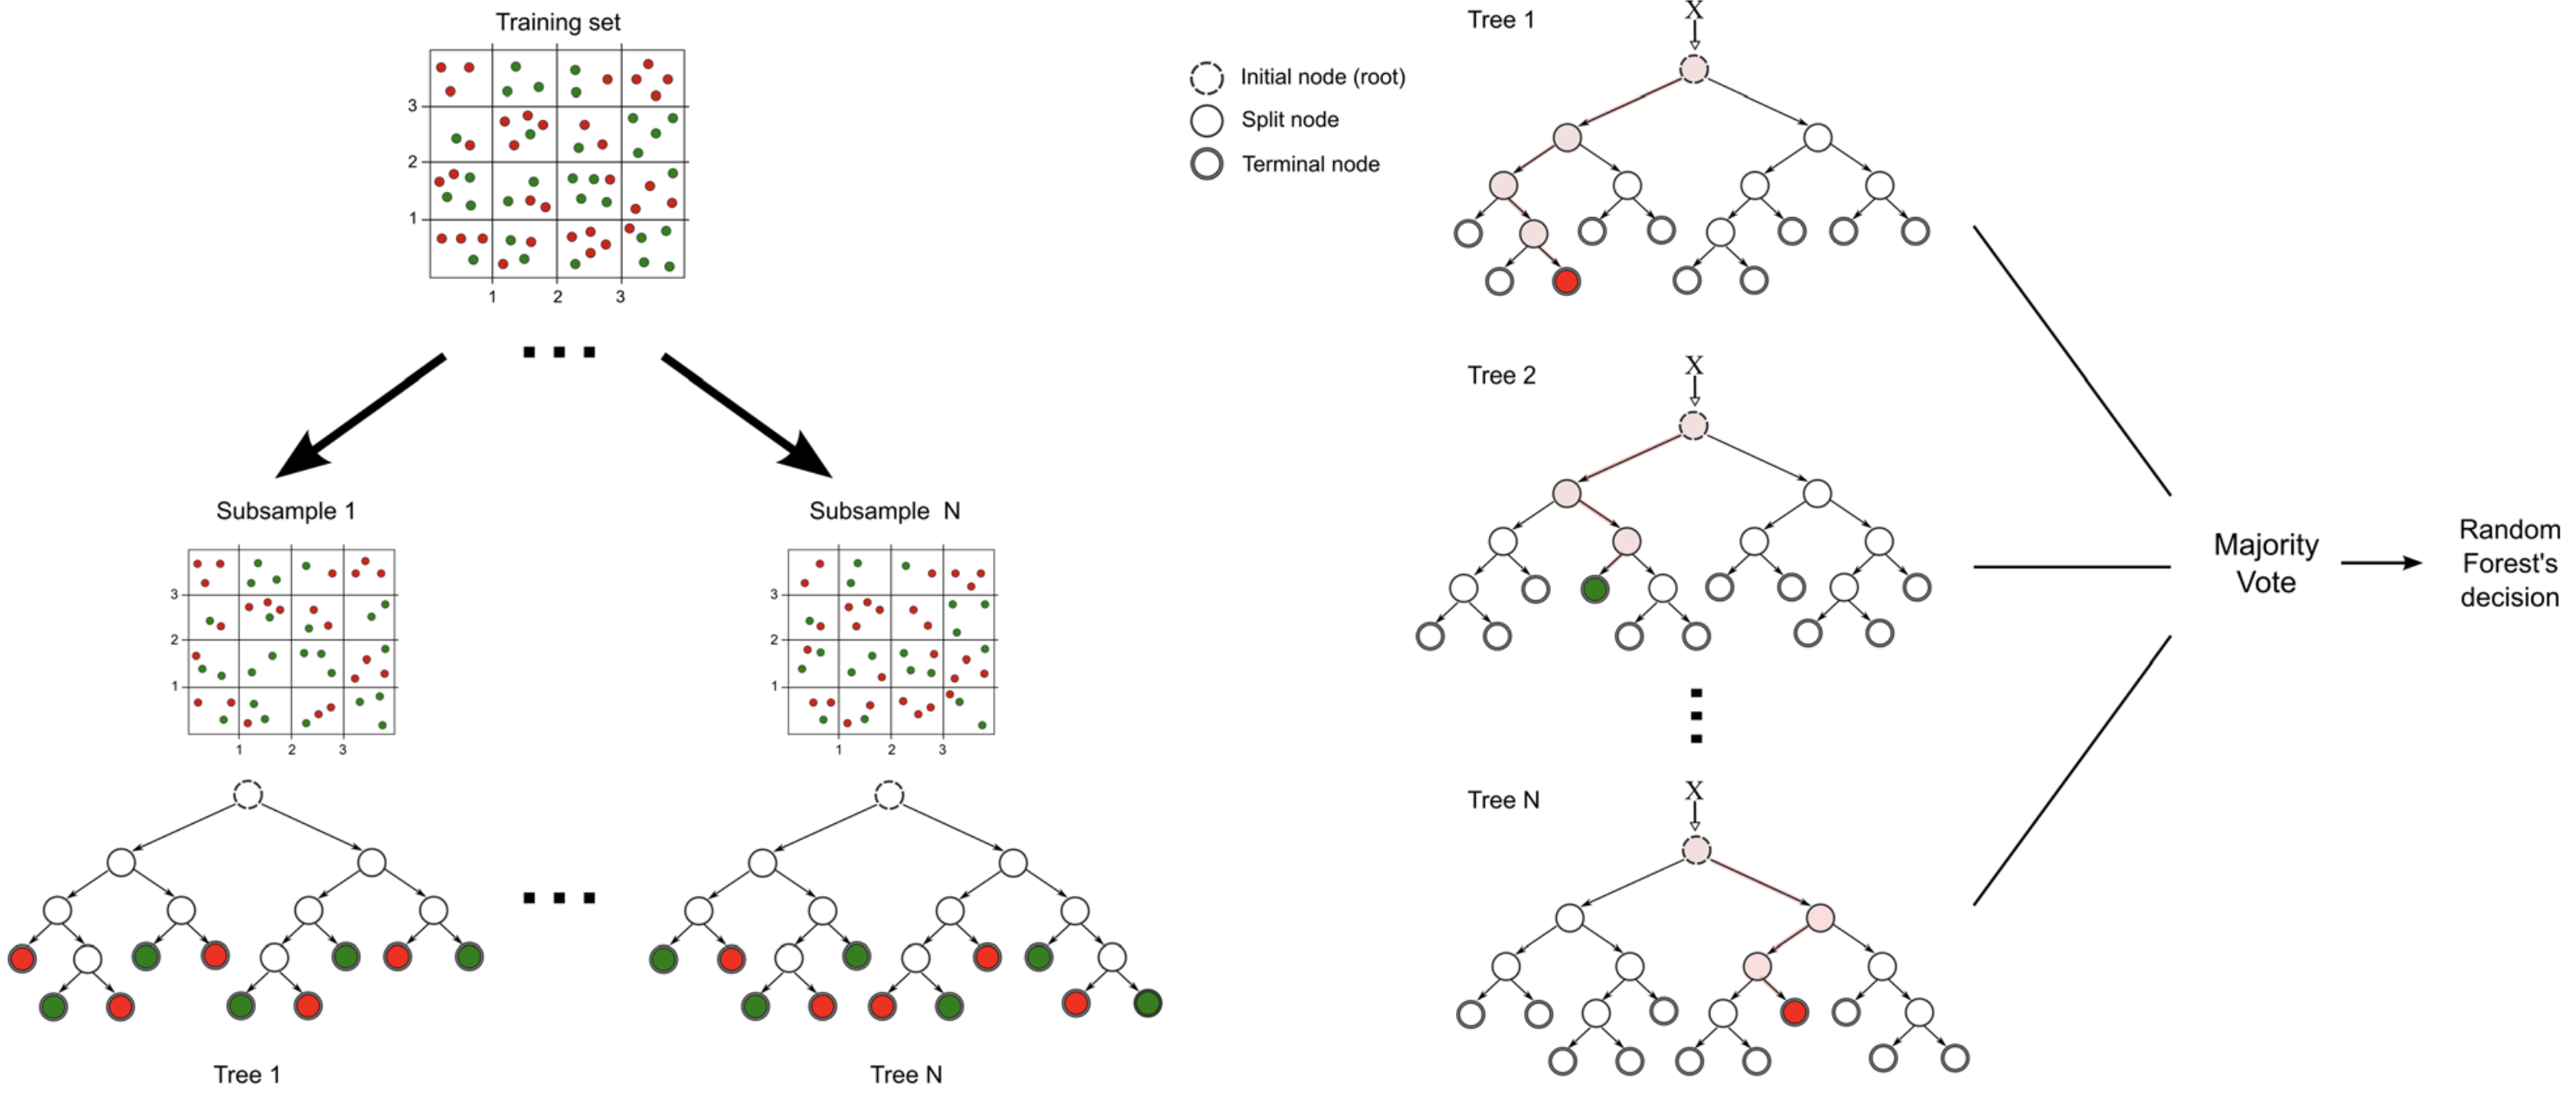
\includegraphics[scale=.27]{fig_random_forest.png}}
    \label{fig:random-forest}
    \legend{Source: ~\citet{Machado2011}}
\end{figure}

Injecting randomness in the procedure through \textit{random feature selection} in node splits can yield benefits in prediction performance including enhancement of generalization capacity and resilience to noise (variance), with overall results comparable to Adaboost (another tree-based ensemble algorithm, but based on boosting)~\cite{Breiman2001}.
Several variations on the classical random forests have been proposed, one of which being the Extremely Randomized Trees~\cite{Geurts2006}.
This algorithm differentiates itself from the others by its approach to node-splitting, which (as the name suggests) strongly randomizes the choice of attribute and cut-point.


\section{Feature Selection Wrappers}

Classification models can be improved upon, in regards to their interpretability and inference capability, by being embedded in a feature selection wrapper algorithm.
Different approaches to this optimization heuristic have been proposed, implemented, and tested.
A common and intuitive approach is Feature Elimination (FE), which has been shown to improve performance and reduce model complexity~\cite{Svetnik2004, Guyon2002}.
It consists of repeatedly eliminating irrelevant features to improve interpretability and performance upon model retraining.
The variable importances can be assessed once, the first time the model is trained, or reassessed each time the model is retrained, configuring a Recursive Feature Elimination (RFE)~\cite{Svetnik2004}.

%Evidence has been found that the learners wrapped RFE are more prone to overfitting \textcolor{red}{\textbf{Svetnik, V}} compared to ones wrapped in the non-recursive variant, although this evidence has been presented as being derived from "limited experience".


\section{Class Imbalance} \label{sec:class_imbalance}

The \textit{class imbalance problem} pervades machine learning research and applications in general~\cite{Chawla2009}.
A consequence of training from datasets skewed towards a majority class, it hinders the performance of classifiers by introducing biases in standard induction algorithms that work best with balanced distributions of classes~\cite{Japkowicz2000}.
This situation consistently manifests itself in medical diagnosis contexts~\cite{Vluymans2019a}, where it is common to have many more examples of some healthy (generally called \textit{negative}) class than the unhealthy (generally called \textit{positive}) one.
Moreover, the domains of application where these skewed distributions arise frequently have an inherently higher cost of mispredictions of the positive minority classes (e.g.\ labeling an ill instance as healthy)~\cite{Kotsiantis2013}.
Nevertheless, many works dealing with applications in mental health do not confer the appropriate attention to the evaluation and treatment of class imbalance~\cite{Burke2019}.
~\citet{Vluymans2019a} separates techniques for the mitigation of class-imbalance effects into four groups: data level preprocessing (\textit{external)}, algorithm-level (\textit{internal}) approaches, and cost-sensitive and ensemble learning.
The two latter are combinations or special applications of the two formers.
While data-level preprocessing consists of modifying the original dataset to have less class imbalance, algorithm-level approaches focus on slightly altering the mechanisms of standard learners to reduce their bias towards the majority class.

Data-level methods can operate by oversampling the minority class, undersampling the majority class, or combining the two.
Undersampling and oversampling can be done randomly or focused~\cite{Kubat1997, Laurikkala2001}, with reportedly mixed results of improvement of one over the other~\cite{Japkowicz2002}.
Oversampling methods work by copying or generating new instances.
In the latter category, the \textit{SMOTE} algorithm~\cite{Chawla2002} reportedly yields considerable performance gains from synthetically creating minority class examples.
In effect, it enlarges decision regions that contain nearby minority class points.

Cost-sensitive learning consists of enhancing the importance of minority classes by altering the amount of cost to different types of errors, classes, or features~\cite{Vluymans2019a}.
One example of this type of approach is MetaCost~\cite{Domingos1999}, which wraps general classifiers training with the introduction of a \textit{cost matrix} that assigns different costs to false positive and false negative errors.

Lastly, in a broad context, ensembles are usually employed for improving accuracy, which by itself would not be of much help for the class imbalance problem.
Thus, ensemble-based solutions for the class imbalance problem introduce specific adaptations, usually done by embedding data-level preprocessing methods or cost-sensitive learning in the induction of the ensemble~\cite{Vluymans2019a}.


\section{Model Evaluation} \label{sec:model-evaluation}

To correctly evaluate the performance of a classification model, it is necessary an understanding of some key concepts, briefly explained in this section.
Evaluation can be done with multiple techniques, assessing different metrics - each having peculiarities in relevance and interpretation depending on the specific context.
Deciding the correct metrics to employ is crucial when dealing with class-imbalanced data because not every metric adequately describes classification quality reliably in this scenario.

\subsection{Evaluation Metrics}\label{subsec:evaluation_metrics}

Since all performance metrics for classifiers correlate to the model's predictions of the labels (or classes) of instances (also called examples), it's useful to employ some common naming of the possible classification cases.
A binary classifier can either predict an instance's label correctly (inferring its true class) or incorrectly (inferring a false class).
When a positive class is inferred correctly, it's called a \textit{true positive}.
Conversely, a misprediction of a positive class is a \textit{false negative}.
The terms \textit{true negative} and \textit{false positive} have analogous definitions.
For convenience, throughout this paper, in the context of some set of predictions, we'll refer to the size of the subsets of \textit{true positives}, \textit{true negatives}, \textit{false positives}, and \textit{false negatives} as \textit{TP}, \textit{TN}, \textit{FP}, and \textit{FN}, respectively.

The first metrics that enable quantitative evaluation of a classifier are its accuracy and error rate.
Both concepts are very intuitive: accuracy is the rate of correct labeling of a set of predictions.
On the other hand, the error rate of this batch of inferences is the frequency of misclassifications.
Accuracy (\textit{Acc}) and error rate (\textit{E}) are therefore correlated (by $Acc = 1 - E$), and can be defined as follows~\cite{Kubat2017}:

\begin{equation}
    Acc = \frac{TP+TN}{TP+TN+FP+FN}
\end{equation}

\begin{equation}
    E = \frac{FP+FN}{TP+TN+FP+FN}
\end{equation}

However, error rate and accuracy are not good estimators for the performance of learners, especially in the presence of class imbalance.
It's easy to see why by imagining the following scenario.
Suppose some model learns from a dataset composed of 80\% negative-class instances (healthy dogs) and 20\% of positive-class instances (diseased dogs).
If measured by accuracy, this learner could be deemed quite successful by always predicting negative labels (asserting that all dogs it analyses are fine).
Yet, that predictor would be disastrous for identifying ill specimens, worse than useless - since animals bearing sickness would not be treated, after confidently being labeled healthy.
Thus, accuracy can mask a learner's problematic performance profile and misjudge its usefulness, especially with imbalanced datasets and false-positive-critical applications - a frequent case in clinical medicine~\cite{Vluymans2019a}.

Alternatively, we could evaluate classification capacity by measuring \textit{precision} (\textit{Pr}) and \textit{recall} (\textit{Re}).
These metrics improve on accuracy by focusing on a class of interest, providing better insight from \textit{TP}, \textit{TN}, \textit{FP}, and \textit{FN}~\cite{Kubat2017}.
Intuitively, precision is the probability that a learner is correct when inferring a positive class, whereas \textit{recall} measures if true positives are identified accordingly.
Depending on the context of the application, one would train its predictor with special attention to one of \textit{precision} or \textit{recall}.
Precision may be more desired in applications where we do not want our model to yield many false positives.
For example, in identifying criminals from pictures, we would not want to accuse innocents.
On the other hand, in studies of clinical conditions, \textit{recall} is generally the most important indicator, since we do not want to miss any positive instance by classifying it as a (false) negative.
We can see that minimizing false positives yields higher precision and minimizing false negatives yields higher recall by analyzing the formulas for these quantities:

\begin{equation}
    Pr = \frac{TP}{TP+FP}
\end{equation}

\begin{equation}
    Re = \frac{TP}{P} = \frac{TP}{TP+FN}
\end{equation}

When a learner changes its profile to be more prone to label instances as positive in general, it will probably increase \textit{recall} at the cost of reduced \textit{precision}.
Thus, a relevant performance metric is the F\textsubscript{\textbeta }-Score, which combines precision and recall in a weighted harmonic mean.
The \textbeta{} factor defines which of the two quantities will have more importance in the measure.
The F\textsubscript{2}-Score is particularly interesting in clinical applications where positive instances are fewer in number and at the same time more important to be noticed (i.e. FNs are more costly).
This is because this metric is affected by changes in the class distribution~\cite{Tharwat2018}, and has an intuitive meaning of its user valuing recall two times more than precision~\cite{C.J.vanRijsbergen1977}.
The F\textsubscript{2}-Score can be reduced to the following equations:

\begin{equation}
    F_2 = \frac{5*TP}{5*TP+4*FN+FP}
\end{equation}

\begin{equation}
    F_2 = \frac{5*Pr*Re}{4*Pr+Re}
\end{equation}

Other important metrics for the medical domain are \textit{sensitivity} and \textit{specificity}.
Although quite traditional to the field, these indicators are rarer in machine learning studies in general~\cite{Kubat2017}.
\textit{Sensitivity} is another name for \textit{recall}, while \textit{specificity} is essentially \textit{recall} for the negative class.
More precisely:

\begin{equation}
    Se = \frac{TP}{P} = \frac{TP}{TP+FN}
\end{equation}

\begin{equation}
    Sp = \frac{TN}{N} = \frac{TN}{TN+FP}
\end{equation}

Just as there is often a trade-off between precision and recall, sensitivity and specificity can vary at odds with each other.
This inference-behavior changes, reflecting the balance between sensitivity and specificity under different hyperparameters, are illustrated by \textit{receiver operating characteristic} (ROC) curves~\cite{Kubat2017}.
These graphs portray sensitivity (also called \textit{true positive rate}) on the y-axis versus a proxy for specificity named \textit{false positive rate} (also called \textit{false alarm rate}) on the x-axis.
The \textit{false positive rate} is defined as~\cite{Fawcett2006}:

\begin{equation}
    Fpr = 1 - Sp = \frac{FP}{N} = \frac{FP}{TN+FP}
\end{equation}

ROC space has some notable points, each translating to a characteristic behavior in classification profile~\cite{Fawcett2006}:
\begin{itemize}
    \item (0,0): to always infer the negative class
    \item (1,1): to always infer the positive class
    \item (0,1): to always infer the correct class
\end{itemize}

%For a given ROC curve, we can identify optimal classifiers by considering only the ROC \textit{convex-hull} (ROCCH), instead of all the available points~\cite{Fawcett2006}.
%These points in the ROC space represent, intuitively, classifiers with lower expected cost, positioned in the northwestern extremities of the graph.
%A classifier is optimal if and only if it lies in the ROCCH~\cite{Fawcett2006}, so we can discard the sub-optimal models and consider only the ones over the convex-hull.
%This graph section is also useful for class imbalance performance assessment.
%Because of the ROC graphs invariance to class imbalance or error costs, one can derive \textit{iso-performance lines}~\cite{Provost2001} and find optimal classifiers over a specific range of the hull for defined class skews and costs.

Based on the analysis of ROC curves, it is customary to consider a classifier's \textit{area under the ROC curve} (\textit{AUC} or \textit{AUCROC}) - a scalar value~\cite{Fawcett2006}.
A perfect classifier will have \textit{AUC}=1, since its ROC curve will be the point (0,1).
The area under the ROC curve can be interpreted as a model's capacity to distinguish instances of different classes as so - it may also be interpreted as the probability of ranking a positive random instance higher than a random negative one~\cite{Fawcett2006}.
It is important to note, however, that the AUCROC is also subject to hiding the true performance of a model under class imbalance, although not as much as accuracy.
With imbalanced classes, a high AUC could merely indicate a better capacity for identifying negative instances~\cite{Burke2019}.

In conclusion, as each approach has its strengths and weaknesses, it is prudent to consider multiple metrics assessments to have a holistic evaluation of classification models.

\subsection{Evaluation Methodologies}\label{subsec:evaluation_methodologies}

With the interest of inducing the best classifier in our reach, we are now ready to consider the methods for using performance metrics to achieve our goal of evaluating and choosing machine learning models.
Several algorithms could be leveraged for that - hence we'll discuss baseline approaches, \textit{random subsampling}, \textit{N-fold Cross-Validation} (CV), and \textit{stratification}.
Nevertheless, The general idea is to perform a \textit{model selection}, choosing the one with parameters that yield the best results, or to perform a final evaluation purely for estimation of performance on unseen data.

The ideal approach for model selection and evaluation would be to separate our dataset into three parts - for training, validation, and tests~\cite{Hastie2009}.
The validation set would be used to assess the performance of models trained with the training set, while testing instances would be reserved for evaluating the chosen best classifier.
There is also the approach to separate the data into only two sets (training and testing)~\cite{Kubat2017}.
Although this could lead to test-error underestimation, this is done to check the generality of the learner~\cite{Hastie2009} - or else we could deem desirable a model overfit to the training data, with no guarantees of extending its prediction capability to new instances.
Both methods are suitable for situations with data abundance.
With smaller datasets, the distribution of instances within each subset is subject to be substantially different from the original dataset~\cite{Kubat2017} - especially with class-imbalanced data.

As an alternative to these standard approaches, one could use \textit{random subsampling} to mitigate the limitations in distribution representation fidelity of the subsets of the baseline methods.
The difference in this procedure is that the training and testing separation is repeated multiple times, each composing different subsets randomly~\cite{Kubat2017}.
This yields, each time, some performance metrics, which are averaged to finish the evaluation.

On the other hand, instead of randomly repeating the training-testing division, the dataset could be divided into K equally-sized parts (also called \textit{folds}, typically 5 or 10).
Then, for each fold, have a round of training, evaluations, and improvements, using the fold as a validation set and the others for training~\cite{Hastie2009}.
One key (advantageous) difference that arises from this approach, called \textit{K-fold cross-validation}, compared to \textit{random subsampling}, is that each of the training sets (and test sets) is disjoint from the others~\cite{Kubat2017}.
This concept can be extended to incorporate a repetition (then being loosely named N-times K-fold cross-validation), where new cutting-points to separate the folds are selected each time, to achieve assessments with more statistical robustness.

Although promising, CV is subject to problems when dealing with highly imbalanced datasets;
the distribution of instances within folds could bear little resemblance to the complete dataset~\cite{Kubat2017}. \textit{Stratified} approaches mitigate this by guaranteeing that all the folds have the same class ratio, respecting the original data's distribution.